\section{Dictionary-Based Compression: The Lempel--Ziv Revolution}

\subsection{Motivation: Hitting the Limits of Statistical Coding}

Statistical coding methods such as Huffman and arithmetic coding achieve near-optimal compression \emph{when the source statistics are known or can be accurately estimated}. However, these methods fundamentally rely on estimating probabilities over symbols or blocks of symbols.

As discussed earlier, block-based statistical coding faces a fundamental dilemma.

\subsubsection{Recap: The Block Coding Dilemma}

Increasing block length allows a coder to better capture dependencies between symbols and approach the entropy rate of the source. However, this comes at a steep cost:
\begin{itemize}
    \item The number of possible blocks grows exponentially with block length.
    \item Estimating probabilities reliably requires exponentially more data.
    \item Memory and computational complexity quickly become impractical.
\end{itemize}

As a result, practical statistical coders are constrained to small contexts and local dependencies.

\subsubsection{The Promise of Exploiting Long-Range Repetition}

Real-world data---text, executable files, logs, DNA sequences---often contains \emph{long-range repetition}. Patterns may repeat far apart, well beyond the reach of fixed-size statistical contexts.

\begin{importantbox}
Statistical coding models \emph{how often} symbols occur, but does not directly model \emph{where long repeated patterns occur}.
\end{importantbox}

This observation motivates a radically different approach to compression.

\subsection{Paradigm Shift: From Statistics to Dictionaries}

Instead of estimating probabilities, dictionary-based compression learns the source \emph{by example}.

\subsubsection{Core Philosophy of Dictionary Coding}

Dictionary-based coders operate on a simple idea:
\begin{quote}
    \emph{Replace repeated substrings by references to earlier occurrences.}
\end{quote}

As the input is processed sequentially, a dictionary of previously seen substrings is constructed. Future occurrences are encoded by references into this dictionary.

\begin{importantbox}
You can think of Lempel--Ziv methods as \emph{learning the source structure rather than estimating probabilities}.
\end{importantbox}

Crucially, the encoder and decoder process the input in exactly the same order and therefore build identical dictionaries \emph{without transmitting the dictionary explicitly}.

\subsubsection{Explicit vs.\ Implicit (Adaptive) Dictionaries}

Dictionary-based methods fall into two categories:
\begin{itemize}
    \item \textbf{Implicit dictionaries}: The dictionary is defined by a sliding window of recent output (e.g., LZ77, LZSS).
    \item \textbf{Explicit dictionaries}: The dictionary is stored and indexed explicitly (e.g., LZ78).
\end{itemize}

We now study the foundational Lempel--Ziv algorithms that underpin modern compression.

\subsection{LZ77: The Sliding Window Algorithm}

Published in 1977 by Abraham Lempel and Jacob Ziv, LZ77 introduced the concept of using recent history as a dictionary.

\subsubsection{The Search Buffer and Look-Ahead Buffer}

LZ77 maintains a sliding window divided into two parts:
\begin{itemize}
    \item \textbf{Search buffer}: Contains the $N$ most recently processed symbols.
    \item \textbf{Look-ahead buffer}: Contains the next $L$ symbols to be encoded.
\end{itemize}

\begin{figure}[H]
    \centering
    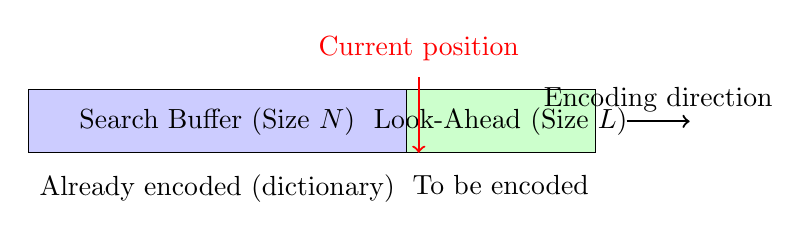
\begin{tikzpicture}[scale=0.8]
        % Search Buffer
        \draw[fill=blue!20] (0,0) rectangle (6,1);
        \node at (3,0.5) {Search Buffer (Size $N$)};
        
        % Look-Ahead Buffer
        \draw[fill=green!20] (6,0) rectangle (9,1);
        \node at (7.5,0.5) {Look-Ahead (Size $L$)};
        
        % Pointer
        \draw[->, thick, red] (6.2,1.2) -- (6.2,0);
        \node[above, red] at (6.2,1.3) {Current position};
        
        % Labels
        \node[below] at (3,-0.2) {Already encoded (dictionary)};
        \node[below] at (7.5,-0.2) {To be encoded};
        
        % Sliding direction
        \draw[->, thick] (9.5,0.5) -- (10.5,0.5);
        \node[above] at (10,0.5) {Encoding direction};
    \end{tikzpicture}
    \caption{LZ77 sliding window structure}
\end{figure}

\subsubsection{Encoding Tuples: (Offset, Length, Next Symbol)}

At each step, the encoder finds the longest match in the search buffer for the prefix of the look-ahead buffer. The match is encoded as:
\[
(\text{offset}, \text{length}, \text{next symbol})
\]
where:
\begin{itemize}
    \item \textbf{Offset}: Distance backward to the match (1-based indexing).
    \item \textbf{Length}: Number of matching symbols.
    \item \textbf{Next symbol}: The first symbol after the match (or EOF).
\end{itemize}

If no match is found, the encoder outputs $(0,0,c)$ where $c$ is the literal symbol from the look-ahead buffer.

\subsubsection{Step-by-Step Encoding Example}

Consider encoding the string \texttt{abracadabra} with a sufficiently large window:

\begin{center}
\begin{tabular}{cccl}
\toprule
Step & Search Buffer & Look-Ahead & Output \\
\midrule
1 & -- & \texttt{abracadabra} & $(0,0,\texttt{a})$ \\
2 & \texttt{a} & \texttt{bracadabra} & $(0,0,\texttt{b})$ \\
3 & \texttt{ab} & \texttt{racadabra} & $(0,0,\texttt{r})$ \\
4 & \texttt{abr} & \texttt{acadabra} & $(3,1,\texttt{c})$ \\
5 & \texttt{abrac} & \texttt{adabra} & $(5,1,\texttt{d})$ \\
6 & \texttt{abraca} & \texttt{abra} & $(7,4,\$)$ \\
\bottomrule
\end{tabular}
\end{center}

Where $\$$ denotes end-of-file. Notice how the second occurrence of "\texttt{abra}" (length 4) is encoded by referencing back to offset 7 (the first occurrence starting at position 1 in our 0-indexed string).

\subsubsection{Decoding Process: Simple Reconstruction}

Decoding is straightforward and proceeds sequentially:

\begin{algorithm}[H]
\caption{LZ77 Decoding}
\begin{algorithmic}[1]
\Procedure{Decode}{$stream$}
    \State Initialize output $\leftarrow$ empty string
    \For{each tuple $(o,l,c)$ in $stream$}
        \If{$o = 0$ and $l = 0$}
            \State Append $c$ to output
        \Else
            \State $start \leftarrow \text{length}(output) - o$
            \For{$i \leftarrow 0$ to $l-1$}
                \State Append output$[start + i]$ to output
            \EndFor
            \If{$c \neq \$ $}
                \State Append $c$ to output
            \EndIf
        \EndIf
    \EndFor
    \State \Return output
\EndProcedure
\end{algorithmic}
\end{algorithm}

\begin{examplebox}
\textbf{Decoding Example}:\\
Decoding the sequence from our example:
\begin{align*}
(0,0,\texttt{a}) &\rightarrow \texttt{a} \\
(0,0,\texttt{b}) &\rightarrow \texttt{ab} \\
(0,0,\texttt{r}) &\rightarrow \texttt{abr} \\
(3,1,\texttt{c}) &\rightarrow \texttt{abrac} \\
(5,1,\texttt{d}) &\rightarrow \texttt{abracad} \\
(7,4,\$) &\rightarrow \texttt{abracadabra}
\end{align*}
\end{examplebox}

\begin{importantbox}
\textbf{Why Decoding Works}: Every referenced symbol has already been reconstructed. The decoder maintains exactly the same output buffer that served as the encoder's search buffer.
\end{importantbox}

\subsubsection{Design Parameters: Window Size and Match Limits}

LZ77 has two key parameters:
\begin{itemize}
    \item \textbf{Search buffer size ($N$)}: Larger buffers find more matches but increase memory and search time.
    \item \textbf{Maximum match length ($L$)}: Limits how far ahead the encoder can look.
\end{itemize}

Practical implementations use efficient data structures (hash tables, suffix arrays) to find matches in $O(1)$ or $O(\log N)$ time rather than the naive $O(NL)$.

\subsection{LZSS: Improving Practical Efficiency}

Published in 1982 by James Storer and Thomas Szymanski, LZSS addresses a key inefficiency in LZ77.

\subsubsection{The Problem with LZ77's Encoding}

LZ77's $(o,l,c)$ format has two inefficiencies:
\begin{enumerate}
    \item \textbf{No-match penalty}: $(0,0,c)$ uses more bits than the literal $c$ alone.
    \item \textbf{Short-match penalty}: Encoding a match of length 2 might not save bits after accounting for tuple overhead.
\end{enumerate}

\subsubsection{Flag Bits: Literal vs. Match}

LZSS introduces a \textbf{flag bit} preceding each encoded element:
\begin{itemize}
    \item \textbf{Flag = 0}: Next item is a literal symbol (8 bits for ASCII).
    \item \textbf{Flag = 1}: Next item is a match pair (offset, length).
\end{itemize}

\begin{importantbox}
\textbf{Key Insight}: LZSS separates the \emph{parsing decision} ("literal or match?") from the \emph{data encoding} itself. This conceptual separation is crucial for understanding modern hybrid compressors.
\end{importantbox}

\begin{figure}[H]
    \centering
    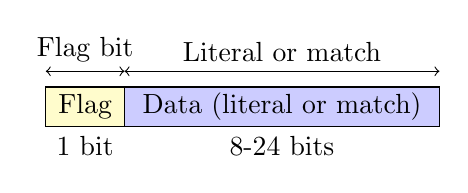
\begin{tikzpicture}
        % Flag bit
        \draw[fill=yellow!20] (0,0) rectangle (1,0.5);
        \node at (0.5,0.25) {Flag};
        
        % Data
        \draw[fill=blue!20] (1,0) rectangle (5,0.5);
        \node at (3,0.25) {Data (literal or match)};
        
        % Labels
        \node[below] at (0.5,0) {1 bit};
        \node[below] at (3,0) {8-24 bits};
        
        \draw[<->] (0,0.7) -- (1,0.7);
        \node[above] at (0.5,0.7) {Flag bit};
        
        \draw[<->] (1,0.7) -- (5,0.7);
        \node[above] at (3,0.7) {Literal or match};
    \end{tikzpicture}
    \caption{LZSS encoding format}
\end{figure}

\subsubsection{Match Threshold}

LZSS introduces a \textbf{match threshold}: only encode matches that are \emph{long enough} to actually save bits. Typically:

\[
\text{Encode match if: } l \times \text{bits\_per\_symbol} > \text{bits\_for\_flag} + \text{bits\_for\_offset} + \text{bits\_for\_length}
\]

For typical parameters (8-bit symbols, 12-bit offset, 4-bit length):
\[
\text{Match if: } l \times 8 > 1 + 12 + 4 = 17 \implies l \geq 3
\]

So LZSS would only encode matches of length 3 or more.

\subsubsection{LZSS Encoding Example}

Let's encode \texttt{abracadabra} with LZSS (match threshold = 3):

\begin{center}
\begin{tabular}{cccc}
\toprule
Step & Look-Ahead & Action & Output \\
\midrule
1 & \texttt{abracadabra} & No match $\geq 3$ & Flag=0, \texttt{a} \\
2 & \texttt{bracadabra} & No match $\geq 3$ & Flag=0, \texttt{b} \\
3 & \texttt{racadabra} & No match $\geq 3$ & Flag=0, \texttt{r} \\
4 & \texttt{acadabra} & Match "\texttt{a}" (length=1) & Flag=0, \texttt{a} \\
5 & \texttt{cadabra} & No match $\geq 3$ & Flag=0, \texttt{c} \\
6 & \texttt{adabra} & Match "\texttt{a}" (length=1) & Flag=0, \texttt{a} \\
7 & \texttt{dabra} & No match $\geq 3$ & Flag=0, \texttt{d} \\
8 & \texttt{abra} & Match "\texttt{abra}" (length=4) & Flag=1, (7,4) \\
\bottomrule
\end{tabular}
\end{center}

Output in binary (simplified):
\begin{itemize}
    \item Flag bits: 0 0 0 0 0 0 0 1
    \item Literals: a b r a c a d
    \item Match: offset=7, length=4
\end{itemize}

\subsubsection{Why LZSS Matters}

\begin{importantbox}
LZSS is the foundation for the \textbf{DEFLATE} algorithm used in ZIP files, gzip, PNG images, and HTTP compression. Its innovations---flag bits and match thresholds---make dictionary compression practical for real-world use.
\end{importantbox}

\subsection{LZ78: The Dictionary Growth Algorithm}

Published in 1978, LZ78 takes a different approach: it builds an explicit dictionary that grows as encoding proceeds.

\subsubsection{Building an Explicit Dictionary from Scratch}

Unlike LZ77's sliding window, LZ78 builds a dictionary of phrases:
\begin{itemize}
    \item Starts with empty dictionary (index 0 represents empty string).
    \item Each new phrase is added to the dictionary.
    \item Dictionary indices are assigned sequentially.
\end{itemize}

\subsubsection{Encoding Pairs: (Dictionary Index, New Symbol)}

LZ78 outputs pairs:
\[
(\text{index}, \text{symbol})
\]
where:
\begin{itemize}
    \item \textbf{Index}: Dictionary index of the longest matching prefix.
    \item \textbf{Symbol}: The next symbol after the match.
\end{itemize}

The new phrase (dictionary[index] + symbol) is added to the dictionary.

\begin{algorithm}[H]
\caption{LZ78 Encoding}
\begin{algorithmic}[1]
\Procedure{Encode}{$input$}
    \State Initialize dict $\leftarrow \{\epsilon\}$ (empty string at index 0)
    \State $current \leftarrow \epsilon$
    
    \For{each symbol $s$ in $input$}
        \If{$current + s$ is in dict}
            \State $current \leftarrow current + s$
        \Else
            \State $i \leftarrow$ index of $current$ in dict
            \State Output $(i, s)$
            \State Add $current + s$ to dict
            \State $current \leftarrow \epsilon$
        \EndIf
    \EndFor
    
    \If{$current \neq \epsilon$}
        \State Output $(index(current), \$)$
    \EndIf
\EndProcedure
\end{algorithmic}
\end{algorithm}

\subsubsection{Worked Example: From String to Codes}

Encoding \texttt{abracadabra}:

\begin{center}
\begin{tabular}{cccc}
\toprule
Step & Current Phrase & Output & New Dictionary Entry \\
\midrule
1 & \texttt{a} & $(0,\texttt{a})$ & 1: \texttt{a} \\
2 & \texttt{b} & $(0,\texttt{b})$ & 2: \texttt{b} \\
3 & \texttt{r} & $(0,\texttt{r})$ & 3: \texttt{r} \\
4 & \texttt{ac} & $(1,\texttt{c})$ & 4: \texttt{ac} \\
5 & \texttt{ad} & $(1,\texttt{d})$ & 5: \texttt{ad} \\
6 & \texttt{abr} & $(1,\texttt{b})$ & 6: \texttt{ab} \\
\bottomrule
\end{tabular}
\end{center}

The output sequence: $(0,a)$, $(0,b)$, $(0,r)$, $(1,c)$, $(1,d)$, $(1,b)$.

\subsubsection{Comparison with LZ77/LZSS}

\begin{importantbox}
\textbf{LZ78 vs LZ77/LZSS}:
\begin{itemize}
    \item \textbf{LZ77/LZSS}: Fast adaptation, limited memory (window), good for local repeats.
    \item \textbf{LZ78}: Slow start, unlimited growth, captures long-term repetitions.
    \item In practice, LZ77/LZSS variants dominate due to better memory behavior and faster adaptation.
\end{itemize}
\end{importantbox}

\subsection{Theoretical Properties: Why Lempel--Ziv Works}

\subsubsection{The Universality Principle}

Lempel--Ziv algorithms have a remarkable theoretical property:

\begin{definitionbox}
\textbf{Universal Compression}: An algorithm is universal if it can compress any stationary ergodic source to its entropy rate \emph{without prior knowledge} of the source statistics.
\end{definitionbox}

Both LZ77 and LZ78 are universal compressors.

\subsubsection{Asymptotic Optimality}

\begin{theorem}[Ziv \& Lempel, 1977-1978]
For any stationary ergodic source with entropy rate $H$, let $L_n$ be the length of the LZ77 or LZ78 encoding of $n$ source symbols. Then:
\[
\lim_{n \to \infty} \frac{\mathbb{E}[L_n]}{n} = H
\]
\end{theorem}

\begin{proof}[Intuition]
As $n$ grows large:
\begin{itemize}
    \item The algorithm sees enough repetitions to build an accurate implicit model.
    \item Common phrases get short codes (through references).
    \item Rare phrases get longer codes (literal transmission).
    \item The average code length approaches the self-information of phrases.
\end{itemize}
\end{proof}

\subsubsection{Practical Implications of Universality}

\begin{importantbox}
\textbf{Why Universality Matters}:
\begin{itemize}
    \item No need to estimate probabilities or build explicit models.
    \item Works on any data type (text, images, executables, DNA).
    \item Adapts automatically to source characteristics.
    \item Explains why LZ methods work so well in practice.
\end{itemize}
\end{importantbox}

\subsection{Bridging Paradigms: Dictionary vs. Entropy Coding}

\subsubsection{Complementary Approaches}

Dictionary coding and entropy coding address different aspects of compression:
\begin{itemize}
    \item \textbf{Dictionary coding}: Exploits \emph{structural redundancy} (repetitions).
    \item \textbf{Entropy coding}: Exploits \emph{statistical redundancy} (skewed symbol frequencies).
\end{itemize}

\subsubsection{The Hybrid Approach}

Modern compressors combine both approaches:

\begin{figure}[H]
    \centering
    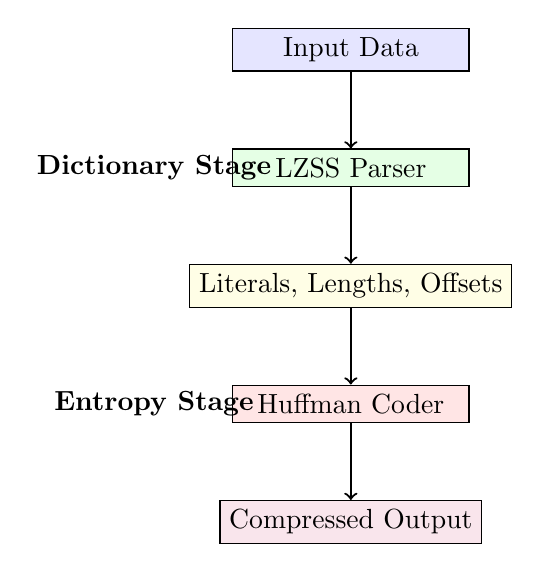
\begin{tikzpicture}[node distance=1.5cm]
        % Nodes
        \node (input) [rectangle, draw, fill=blue!10, minimum width=3cm] {Input Data};
        \node (lzss) [rectangle, draw, fill=green!10, minimum width=3cm, below of=input] {LZSS Parser};
        \node (stream) [rectangle, draw, fill=yellow!10, minimum width=3cm, below of=lzss] {Literals, Lengths, Offsets};
        \node (huffman) [rectangle, draw, fill=red!10, minimum width=3cm, below of=stream] {Huffman Coder};
        \node (output) [rectangle, draw, fill=purple!10, minimum width=3cm, below of=huffman] {Compressed Output};
        
        % Arrows
        \draw[->, thick] (input) -- (lzss);
        \draw[->, thick] (lzss) -- (stream);
        \draw[->, thick] (stream) -- (huffman);
        \draw[->, thick] (huffman) -- (output);
        
        % Labels
        \node[left of=lzss, xshift=-1cm] {\textbf{Dictionary Stage}};
        \node[left of=huffman, xshift=-1cm] {\textbf{Entropy Stage}};
    \end{tikzpicture}
    \caption{Hybrid compression pipeline (e.g., DEFLATE algorithm)}
\end{figure}

The DEFLATE algorithm (used in ZIP, PNG, gzip) works precisely this way:
\begin{enumerate}
    \item LZSS finds repeated strings, outputs literals and matches.
    \item Huffman coding compresses:
    \begin{itemize}
        \item Literal symbols (0-255)
        \item Match lengths (257-285)
        \item Match distance codes (0-29)
    \end{itemize}
\end{enumerate}

\subsection{Summary and Forward Look}

\subsubsection{Key Takeaways}

\begin{itemize}
    \item \textbf{Paradigm shift}: Dictionary coding exploits repetition rather than probabilities.
    \item \textbf{LZ77}: Sliding window approach, encodes matches as triples.
    \item \textbf{LZSS}: Practical improvement with flag bits and match thresholds.
    \item \textbf{LZ78}: Explicit dictionary growth, encodes pairs.
    \item \textbf{Universality}: LZ methods work on any stationary source without prior knowledge.
    \item \textbf{Modern practice}: Hybrid systems (LZSS + Huffman) dominate.
\end{itemize}

\subsubsection{The Road Ahead: DEFLATE and Beyond}

In our next lecture, we'll study the DEFLATE algorithm in detail:
\begin{itemize}
    \item How LZSS and Huffman coding are combined.
    \item The gzip/ZIP/PNG compression pipeline.
    \item Practical implementation considerations.
    \item Performance trade-offs and optimizations.
\end{itemize}

\begin{importantbox}
\textbf{Historical Context}: The Lempel--Ziv papers (1977, 1978) are among the most cited in information theory. Their algorithms underpin much of today's digital compression infrastructure. Understanding these foundations is essential for working with modern compression standards.
\end{importantbox}

% ================= END OF CHAPTER EXERCISES =================

\subsection*{End of Chapter Exercises}

\begin{exercisebox}
\textbf{Exercise 5.1 (LZ77 Encoding)}\\
Encode the string \texttt{TOBEORNOTTOBEORTOBEORNOT} using LZ77 with a search buffer of size 12. Show your work step by step with the search buffer, look-ahead buffer, and output tuples.
\end{exercisebox}

\begin{exercisebox}
\textbf{Exercise 5.2 (LZSS Efficiency Analysis)}\\
Compare LZ77 and LZSS for encoding a sequence with parameters: 8-bit symbols, 12-bit offsets, 4-bit lengths.
\begin{enumerate}[label=(\alph*)]
    \item How many bits does LZ77 use for a non-match?
    \item How many bits does LZSS use for a literal?
    \item What is the minimum match length that saves bits in LZSS?
    \item When would LZ77 be more efficient than LZSS?
\end{enumerate}
\end{exercisebox}

\begin{exercisebox}
\textbf{Exercise 5.3 (LZ78 Dictionary Growth)}\\
Encode the string \texttt{ABABABABA} using LZ78. Show the dictionary after each step and the complete output sequence. How many dictionary entries are created?
\end{exercisebox}

\begin{exercisebox}
\textbf{Exercise 5.4 (Algorithm Comparison)}\\
For each string below, predict which would perform better: LZ77/LZSS or LZ78? Explain why.
\begin{enumerate}[label=(\alph*)]
    \item \texttt{AAAAAAAAAAAAAAAAAAAA} (20 A's)
    \item \texttt{ABCDEFGHIJKLMNOPQRSTUVWXYZ}
    \item \texttt{ABABABABABABABABABAB}
    \item A file containing the same 1KB block repeated 100 times
\end{enumerate}
\end{exercisebox}

\begin{exercisebox}
\textbf{Exercise 5.5 (Decoding Challenge)}\\
Decode the following LZSS encoded sequence (match threshold = 3):
\begin{verbatim}
0 T
0 H
0 E
1 (3,5)
0 _
0 _
1 (5,4)
0 .
\end{verbatim}
Where: 
- Each line represents one encoded element
- Flag 0 indicates a literal character
- Flag 1 indicates a match (offset, length)
- \_ represents space character
- . represents period

What is the original string? Show your decoding step by step.
\end{exercisebox}

\begin{exercisebox}
\textbf{Exercise 5.6 (Window Size Analysis)}\\
Consider LZ77 with search buffer size $N$.
\begin{enumerate}[label=(\alph*)]
    \item How many bits are needed to encode an offset value?
    \item If we increase $N$ from 4096 to 65536, how many more bits are needed for offsets?
    \item What is the trade-off in choosing $N$?
    \item In practice, why might we choose $N = 32768$ over $N = 65536$ even if memory is available?
\end{enumerate}
\end{exercisebox}

\begin{exercisebox}
\textbf{Exercise 5.7 (Universal Compression Intuition)}\\
Explain in your own words why Lempel--Ziv algorithms are universal. Why don't they need to know source statistics in advance? How do they "learn" the source structure?
\end{exercisebox}

\begin{exercisebox}
\textbf{Exercise 5.8 (Hybrid Coding Design)}\\
Design a simple hybrid compressor that:
\begin{enumerate}[label=(\alph*)]
    \item Uses LZSS with match threshold 3
    \item Collects statistics on literals, lengths, and offsets
    \item Applies Huffman coding to each alphabet separately
\end{enumerate}
How would the decoder know which Huffman trees to use?
\end{exercisebox}

\begin{exercisebox}
\textbf{Exercise 5.9 (Search Efficiency)}\\
A naive LZ77 implementation searches for matches by comparing the look-ahead buffer against every position in the search buffer.
\begin{enumerate}[label=(\alph*)]
    \item What is the time complexity of this approach?
    \item Describe how a hash table can improve search efficiency.
    \item What information would you store in the hash table?
    \item How would you handle hash collisions?
\end{enumerate}
\end{exercisebox}

\begin{exercisebox}
\textbf{Exercise 5.10 (Theoretical Limits)}\\
Prove or provide intuition for:
\begin{enumerate}[label=(\alph*)]
    \item LZ77 cannot achieve compression ratio better than the entropy rate for i.i.d. sources.
    \item LZ78 may perform poorly on very short inputs.
    \item For sources with long-range dependencies, LZ methods can outperform block Huffman coding even with large blocks.
\end{enumerate}
\end{exercisebox}
